\documentclass[10pt,a4paper]{article}
\usepackage[utf8]{inputenc}
\usepackage[spanish]{babel}
\usepackage[margin=1in]{geometry}
\usepackage{amsmath}
\usepackage{amsfonts}
\usepackage{amssymb}
\usepackage{enumitem}
\usepackage{hyperref} 
\usepackage{graphicx}
\usepackage{url}
\usepackage{breakurl}
\hypersetup{pdftex,colorlinks=true,allcolors=black}
\hypersetup{
    pdftitle={},
    pdfauthor={Pablo Riutort Grande},
    pdfsubject={},
    bookmarksnumbered=true,     
    bookmarksopen=true,         
    bookmarksopenlevel=1,       
    colorlinks=true,            
    pdfstartview=Fit,           
    pdfpagemode=UseOutlines,    % this is the option you were lookin for
    pdfpagelayout=TwoPageRight
}
\usepackage{listings}
\usepackage{xcolor}
\usepackage{hypcap}
\definecolor{codegreen}{rgb}{0,0.6,0}
\definecolor{codegray}{rgb}{0.5,0.5,0.5}
\definecolor{codepurple}{rgb}{0.58,0,0.82}
\definecolor{backcolour}{rgb}{0.95,0.95,0.92}
\lstdefinestyle{mystyle}{
    backgroundcolor=\color{backcolour},   
    commentstyle=\color{codegreen},
    keywordstyle=\color{magenta},
    numberstyle=\tiny\color{codegray},
    stringstyle=\color{codepurple},
    basicstyle=\ttfamily\footnotesize,
    breakatwhitespace=false,         
    breaklines=true,                 
    captionpos=b,                    
    keepspaces=true,                 
    numbers=left,                    
    numbersep=5pt,                  
    showspaces=false,                
    showstringspaces=false,
    showtabs=false,                  
    tabsize=2
}
\lstset{style=mystyle}
\usepackage{xparse}
\usepackage{verbatim}
\NewDocumentCommand{\codeword}{v}{%
\texttt{{#1}}
}
\author{Pablo Riutort Grande}
\title{
	Seguridad y pentesting de servidores de datos\\
	\vspace{0.5cm}
	PEC 2\\
	\vspace{1cm}
	\textbf{Arquitectura de las aplicaciones web}
	\vspace{1cm}\\UOC - MISTIC
}

\begin{document}
\maketitle
\pagebreak
\tableofcontents
\listoffigures
\pagebreak

\section{Resumen ejecutivo}
\begin{comment}
En este apartado se debe explicar de manera clara y
precisa todos los aspectos relevantes hallados sobre la arquitectura del Portal
de la UOC y las medidas de seguridad presentes. Se recomienda también
seguir una cierta organización lógica al presentar los resultados (capa de red,
capa de aplicación, etc...).
\end{comment}

Se ha hecho un análisis del portal de la universidad de la UOC de manera pasiva para determinar las medidas de seguridad presentes y otras características.

\subsubsection{Capa de red}
A nivel de red el sitio se mueve en el rango de IPs 213.73.40.0/24 con algunas aplicaciones abiertas y otras filtradas:

\begin{center}
\begin{tabular}{|c|c|c|c|c|c|c|}
\hline 
 \textbf{Puerto} & \textbf{Servicio} \\ 
\hline 
 22 & ssh \\ 
\hline 
 25 & smtp \\ 
\hline 
 515 & printer \\ 
\hline 
 3306 & mysql \\ 
\hline 
 53 & domain \\ 
\hline 
 8400 & cvd (servicios de backup)\\ 
\hline 
 8402 & abarsd (servicios de backup)\\ 
\hline
 6881 & bittorrent-tracker \\
\hline 
 ... & ... \\
\hline 
\end{tabular} 
\end{center}

En el rango de IPs se han encontrado un total de 23 hosts, entre algunos de ellos están los servidores de DNS y de correo:
\begin{itemize}
\item portugal.uoc.es (213.73.40.8)
\item tibet\_dnsex.uoc.es (213.73.40.9)
\item nepal\_dnsex.uoc.es (213.73.40.10)
\item tibet.uoc.es (213.73.40.45) (Servidor de DNS)
\item tibet\_dns.uoc.es (213.73.40.46)
\item nepal.uoc.es (213.73.40.47) (Servidor de DNS)
\item nepal\_dns.uoc.es (213.73.40.48)
\item croacia\_campus.uoc.es (213.73.40.49)
\item www.uoc.edu (213.73.40.210)
\item cv.uoc.edu (213.73.40.211)
\item 73-40-242.uoc.es (213.73.40.242)
\item eduroam.uoc.edu (213.73.40.249)
\item ...
\item aspmx5.googlemail.com	(Correo)
\item aspmx.l.googlemail.com (Correo)
\item ...
\end{itemize}

\subsubsection{Capa de aplicación}
La aplicación utiliza varias tecnologías, entre ellas se han encontrado evidencias de:
\begin{itemize}
\item Librerías y Frameworks: jQuery, Mustache, WordPress
\item Apache y algunos módulos del mismo (ModLayout)
\item Analíticas: Google Analytics, Hotjar
\item Lenguajes: PHP, Python, JavaScript y MySQL
\item Uso de cifrado SSL: Se usa la redirección del tráfico http a https.
\item Sistemas operativos: Ubuntu, Debian
\item Gestores de tráfico (f5 Big-IP).
\end{itemize}

\textbf{Vulnerabilidades}\\
En ese nivel se han encontrado algunas vulnerabilidades o malas configuraciones que pueden ser explotables, algunas son:
\begin{itemize}
\item Se han encontrado direcciones de correo en el sistema que se sabe que pertenecen a fugas de información.
\item Vulnerabilidades conocidas de Apache recogidas en CVE (CVE-2017-7679, CVE-2017-9798...)
\item Headers mal configurados con riesgos de clickjacking y cross-site-scripting.
\item Cookies atributos ausentes, sin flags de seguridad o con sobreinformación.
\end{itemize}

\section{Metodología utilizada}
\begin{comment}
En este apartado se debe explicar la metodología y
herramientas utilizadas para la elaboración de la PEC. A la vez que se explica
cómo se han realizado las pruebas.
\end{comment}
La metodología utilizada ha sido la recomendada por la OWASP en su guía de \textit{Testing Information Gathering} (OTG-INFO)\cite{owasp}. Siguiendo esta guía de forma libre se ha realizado un análisis pasivo del portal web de esta universidad (\url{www.uoc.edu}) y extraído información información de la misma.\\

A continuación se describe en más detalle este análisis siguiendo los apartados de la guía.
\subsection{Búsqueda mediante motores de búsqueda para el descubrimiento de fugas de información (OTG-INFO-001)}
\label{OTF-INFO-001}
Este primer paso de la guía consiste en recabar información del sitio utilizando motores de búsqueda y operadores especiales que nos permiten acceder a funcionalidades avanzadas.\\ Concretamente hemos utilizado el operador \textbf{site:uoc.edu} que restringe los resultados de la búsqueda al dominio de la página que nos interesa analizar [Ver \ref{ann:otg-info-001}].\\
Existen ciertas páginas que normalmente no aparecerían en una búsqueda convencional, pero si aplicamos los operadores podemos sacar información interesante, como es el caso de la página \url{http://lpg.uoc.edu/IATE/} que se ha encontrado mediante el operador \textbf{site:uoc.edu intitle:``index of''} [Fig. \ref{fig:otg-info-001-2}].

\subsection{Fingerprint del servidor web (OTG-INFO-002)}
Este paso consiste en averiguar el tipo y versiones del servidor web. La idea es observar los datos de las cabeceras que devuelva el servidor\\

Shodan es un motor de búsqueda especializado en dispositivos conectados a internet \cite{shodan}. Podemos utilizar este motor para hacer una búsqueda especializada de la página de UOC en el puerto 80 ``\textbf{hostname:uoc.edu port:80}'' y obtener información sobre los dispositivos que tengan que ver con este dominio [Fig. \ref{fig:otg-info-002-1}].  Shodan nos enseña la cabecera de las respuestas del servidor y nos pone qué software utiliza el servidor web: Apache/2.4.18 y Sistema operativo Ubuntu [Fig. \ref{fig:otg-info-002-2}]. Además, entre los dispositivos se han encontrado evidencias de otras tecnologías como jQuery Migrate, Wordpress, PHP y MySQL así como algunas vulnerabilidades conocidas [Fig. \ref{fig:otg-info-002-2}].\\

Otra herramienta que se ha utilizado es Netcraft que nos da un análisis muy variado del dominio introducido como la dirección IP, dónde está hosteada la red, qué trackers tiene y algunas tecnologías que se utilizan en el servidor [Fig. \ref{fig:otg-info-002-3}].\\

Finalmente, hemos visto que el dominio www.uoc.edu redirige el tráfico a https, vale la pena inspeccionar los certificados que se intercambian con el dominio con el comando
\begin{lstlisting}[language=bash]
openssl s_client -connect uoc.edu:443
\end{lstlisting}
Vemos que en la respuesta se produce un handshake satisfactorio y nos devuelve el certificado del servidor para proceder con la conexión de manera segura.

\subsection{Revisión de metadatos en busca de fuga de información (OTG-INFO-003)}
Este apartado consiste en revisar datos del servidor para entender qué paths (o rutas) tiene actualmente. Para esto, un archivo muy útil suele ser el robots.txt ya que indica a los buscadores qué rutas no tienen que se indexadas por los buscadores. Podemos descargar este fichero con el comando wget y observar una primera vista de las aplicaciones que esconde el dominio [Ver \ref{ann:otg-info-003}].\\
Otra acción que se recomienda en este paso es consultar los metadatos de la página, para eso podemos consultar los tags META de la sección HEAD del documento HTML.

\subsection{Enumeración de aplicaciones en el servidor web (OTG-INFO-004)}
Se ha utilizado la herramienta SpiderFoot para hacer una búsqueda sobre el dominio. SpiderFoot permite el descubrimiento de los recursos que pertenecen a un dominio y monitorizarlos \cite{spiderfoot}. Se ha realizado un scanner de tipo footprint que consiste en entender el perímetro de la red del objetivo, las entidades asociadas y otra información, en cambio, el pasivo pretende recopilar tanta información como sea posible sin tocar el objetivo o sus afiliados [Ver \ref{fig:otg-info-004-1}].\\
Para este paso también se ha utilizado la herramienta llamada Maltego, la cual genera un grafo de entidades y conexiones entre ellas a través de un dominio dado \cite{maltego}. Mediante este grafo podemos sacar mucha información precisa y la relación que hay entre las entidades de manera catalogada: Servidores de DNS, servidores de correo, direcciones, personas, etc.\\
Finalmente, la guía también recomienda el uso de Nikto para detectar vulnerabilidades conocidas en servidores web \cite{nikto}. Con esta herramienta podemos ver que existen riesgos de clickjacking y cross-site-scripting debido a la mala configuración de headers.

A través de la información que hemos obtenido hasta ahora se puede realizar un escaneo aún más exhaustivo con nmap. Nmap es una herramienta de exploración de puertos y escáner con múltiples opciones \cite{nmap}. Para este ejercicio se ha ejecutado el comando sobre el rango de IPs encontrado con Maltego [Ver \ref{ann:nmap}].
\begin{lstlisting}
nmap 213.73.40.0/24
\end{lstlisting}
Este comando nos da mucha información de todas las IPs del rango como distintas aplicaciones en distintos servidores como impresoras, protocolos de correo, ftp, ssh, etc.

\subsection{Mapear rutas de ejecución a través de la aplicación (OTG-INFO-007)}
Este proceso consiste en entender la estructura de la aplicación y su disposición en la red. Para este paso se ha utilizado ZAP (Zed Attack Proxy). ZAP es una herramienta de pentesting de OWASP diseñada para testear aplicaciones web \cite{zap}.
Con esta herramienta podemos automatizar el proceso de descubrimiento de URLs de forma sencilla mediante spiders que recorren el dominio, ZAP registra la URL, el método utilizado (Verbo HTTP), la request enviada y la response. De esta forma, se consigue un mapa de toda la aplicación y sus rutas [Ver \ref{ann:otg-info-007}].\\
ZAP, además, catalogará los diferentes niveles de riesgo que se haya podido encontrar [Ver. \ref{fig:otg-info-007-2}]; entre ellos ha encontrado mala configuración del cross domain, mala configuración de cookies, headers ausentes, etc.

\subsection{Fingerprint del framework de la aplicación (OTG-INFO-008)}
Esta tarea consiste en intenta averiguar el framework que se esté utilizando en el servidor web para la aplicación. Típicamente las aplicaciones basadas en web utilizan frameworks para facilitar tareas que de otra forma serían muy costosas de desarrollar y mantener, sin embargo, con estos frameworks también existen riesgos de seguridad que vale la pena conocer y mitigar. Conocer también las configuraciones típicas de este framework para saber si se han realizado correctamente es un proceso importante para el fingerprinting.\\
Para este paso se ha utilizado la herramienta Whatweb que reconocerá las tecnologías utilizadas en el servidor web tales como CMS o librerías de JavaScript \cite{whatweb}, en el caso de la página de la UOC ha encontrado [Ver \ref{fig:otg-info-008-1}]:
\begin{itemize}
\item Se trata de un servidor Apache
\item Hay una mención a un framework llamado ModLayout. Esto lo sabemos por el header no estándard de ``X-Powered-By'' típicamente designado para esto \cite{x-pow}.
\item Se trata de un servidor F5-BigIP.
\end{itemize}
Finalmente, se ha utilizado la herramienta Wappalyzer para identificar otras tecnologías que se puedan estar utilizando \cite{wappalyzer}. En la página de la UOC se ha encontrado el uso de la librería jQuery y el framework JavaScript de Mustache [Ver \ref{fig:otg-info-008-2}].

\subsection{Fingerprint de la aplicación (OTG-INFO-009)}
Conocer los componentes de la aplicación que se está testeando es también importante y reduce el esfuerzo de un test más exhaustivo puesto que se tiene una idea de los componentes de la aplicación.\\
Para entender la aplicación un buen sitio donde mirar son las cookies que genera la aplicación y buscar pistas en el código HTML.\\
En las cookies podemos observar la presencia de las aplicaciones de análisis de Hotjar y Google Analytics \cite{gaq} [Ver \ref{fig:otg-info-009}]. Existen cookies propias que dan pistas de la naturaleza de la aplicación que presenta el servidor web, como la llamada \_\_utmv cuyo valor describe al tipo de usuario que utiliza la aplicación (TipusUsuari=UOC\%2FESTUDIANT).\\
En cuanto al análisis del código HTML no se han encontrado pistas o patrones que delaten a un framework o describan una apliación.\\

\pagebreak
\section*{Anexo}
\appendix
\section{Evidencias}
\label{ann:evidencias}
\begin{comment}
A modo de anexo, en este último apartado se deberán exponer las
capturas de pantalla u otras evidencias halladas mediante a la aplicación de la
metodología expuesta en el apartado 2 que soporten las conclusiones
establecidas en el apartado 1. Importante: Se deben añadir únicamente
evidencias relevantes evitando añadir capturas u otra información que no sea
útil.
\end{comment}

\subsection{OTG-INFO-001}
\label{ann:otg-info-001}
\begin{figure}[ht!]
\centering
  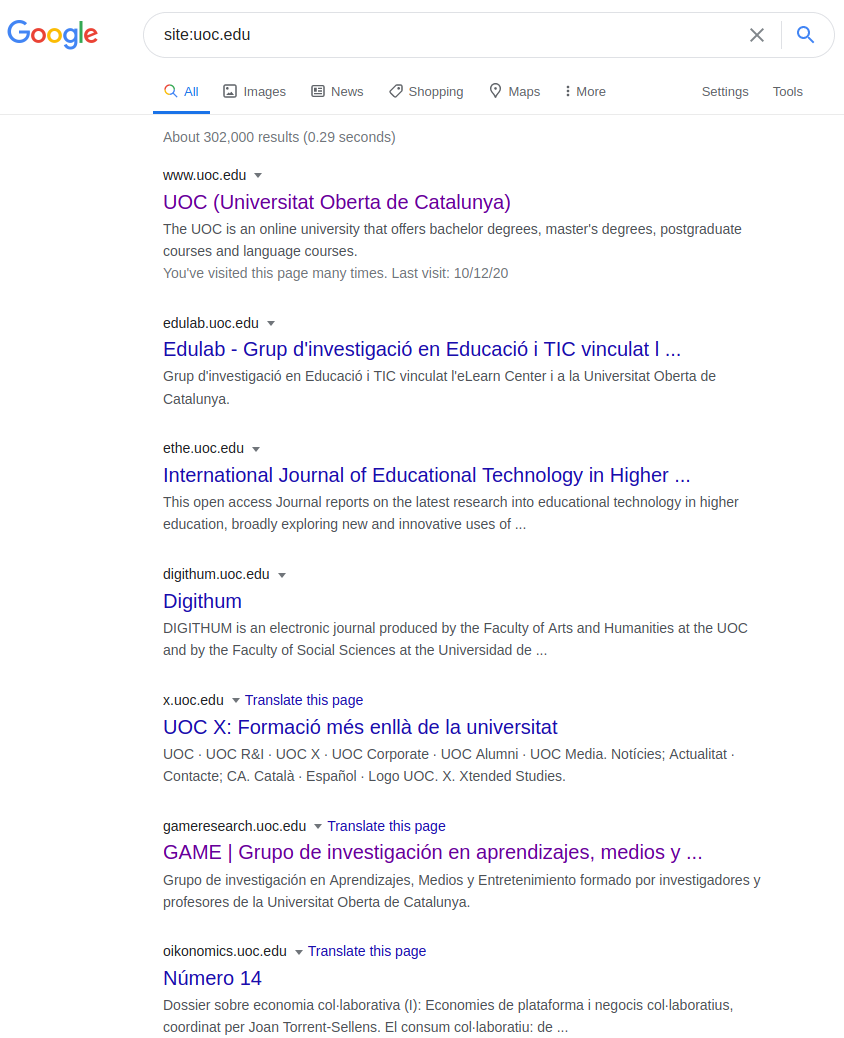
\includegraphics[scale=0.27]{google.png}
  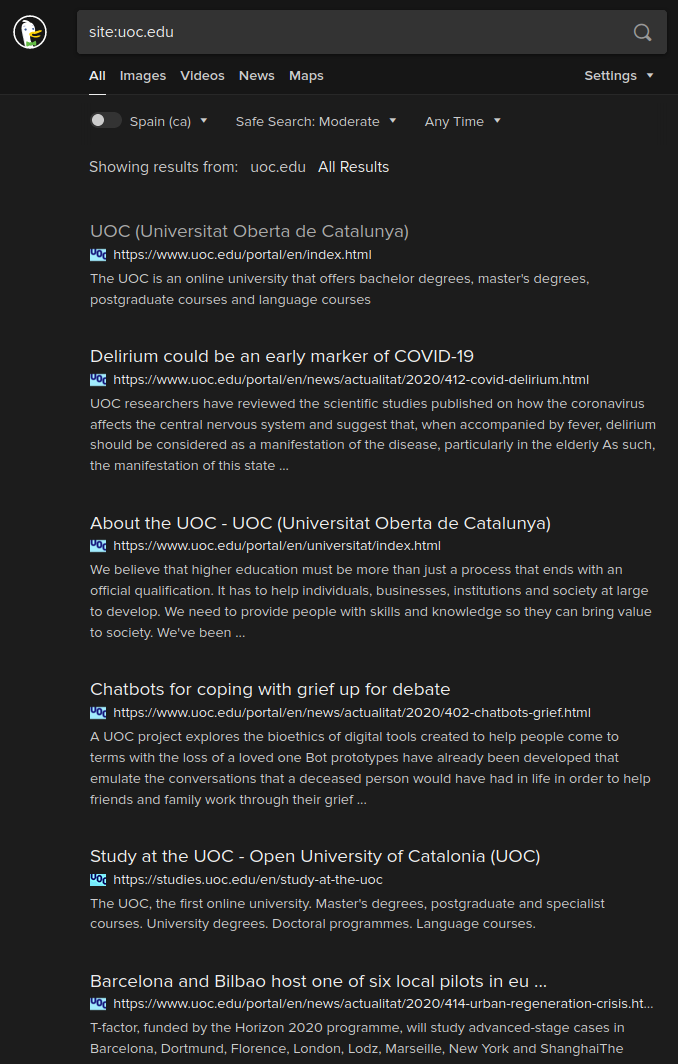
\includegraphics[scale=0.27]{ddg.png}\\
  \hspace*{0.5in}
  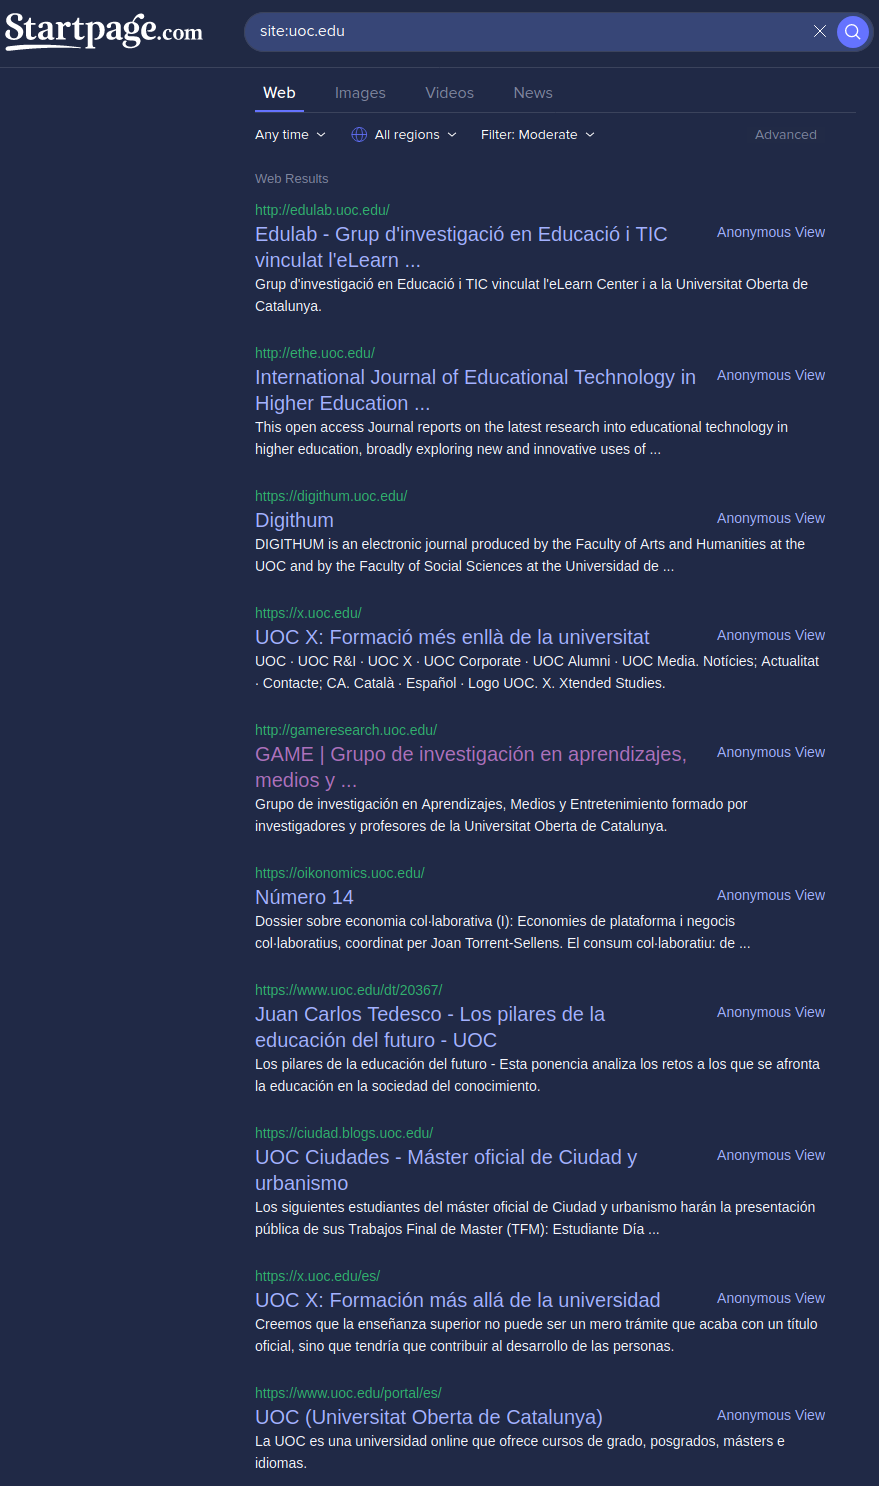
\includegraphics[scale=0.2]{startpage.png}
  \caption{Operador ``site: uoc.edu'' con Google, Duck Duck Go y Startpage.com}
  \label{fig:otg-info-001-1}
\end{figure}

\pagebreak

\begin{figure}[ht!]
\centering
  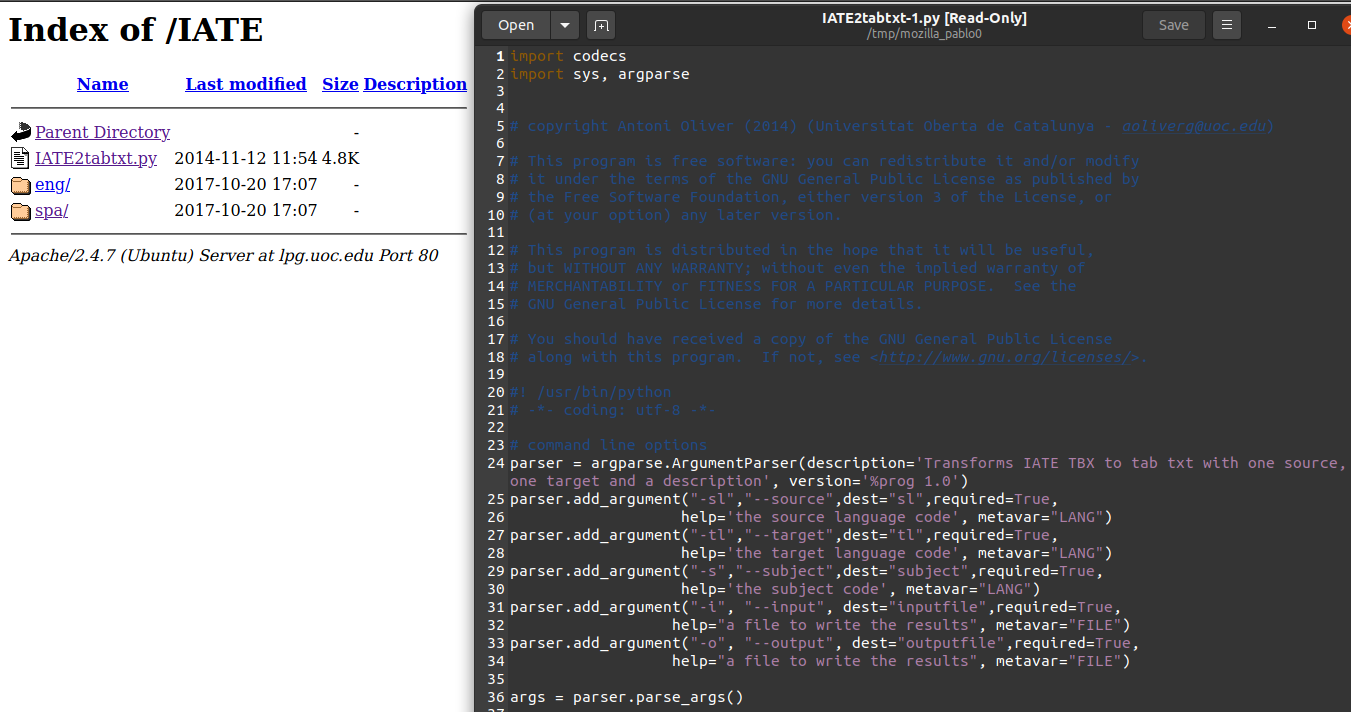
\includegraphics[scale=0.2]{dorks.png}
  \caption{Mediante el operador site:uoc.edu intitle:``index of'' podemos encontrar varios archivos del servidor e incluso scripts}
  \label{fig:otg-info-001-2}
\end{figure}

\pagebreak

\subsection{OTG-INFO-002}
\label{ann:otg-info-002}
\begin{figure}[h!]
  \centering
  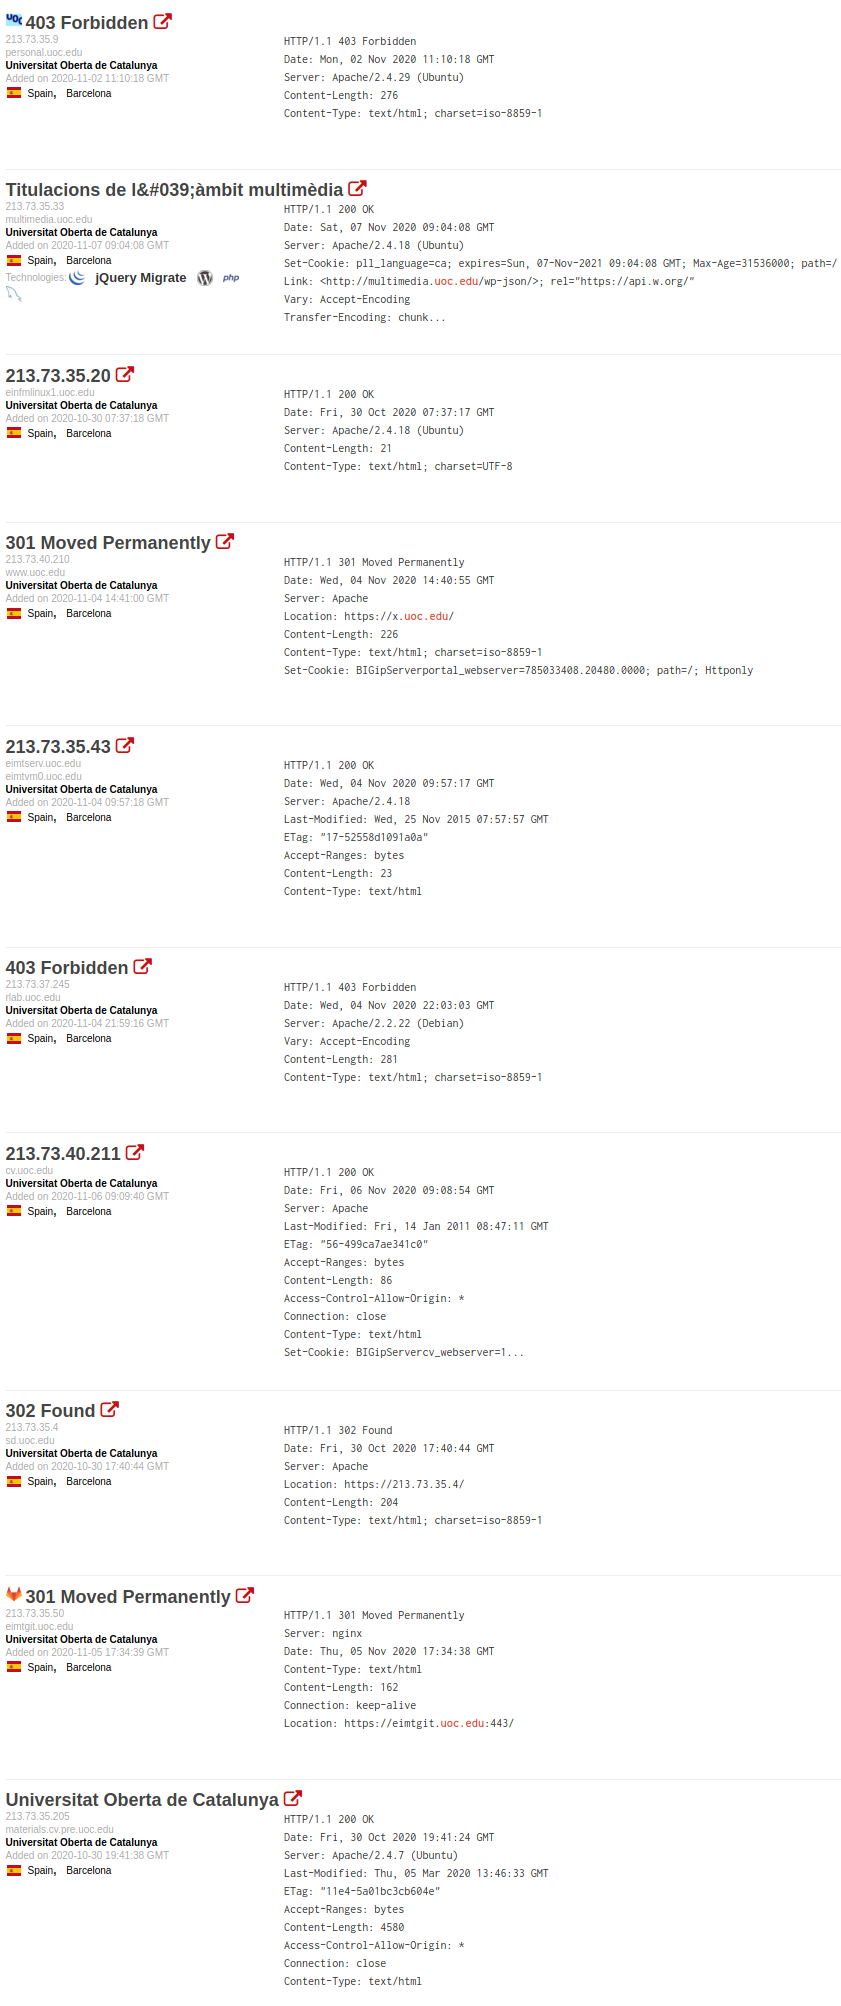
\includegraphics[scale=0.25]{shodan1.png}
  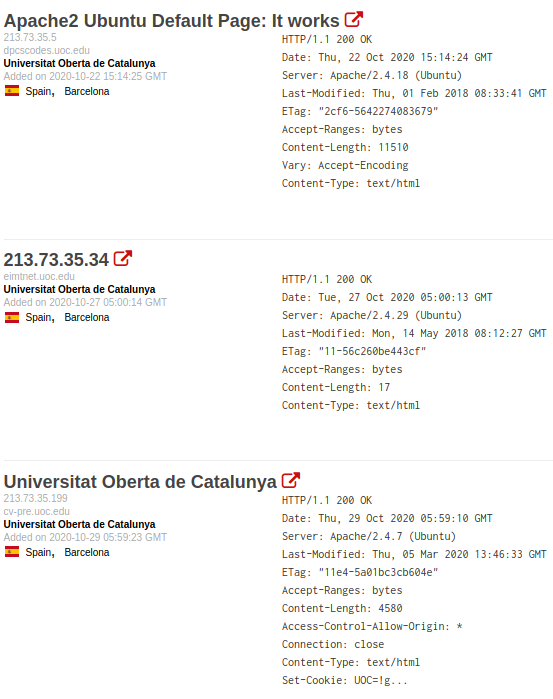
\includegraphics[scale=0.25]{shodan2.png}
  \caption{Detalle de resultados con Shodan}
  \label{fig:otg-info-002-1}
\end{figure}

\begin{figure}[h!]
  \centering
  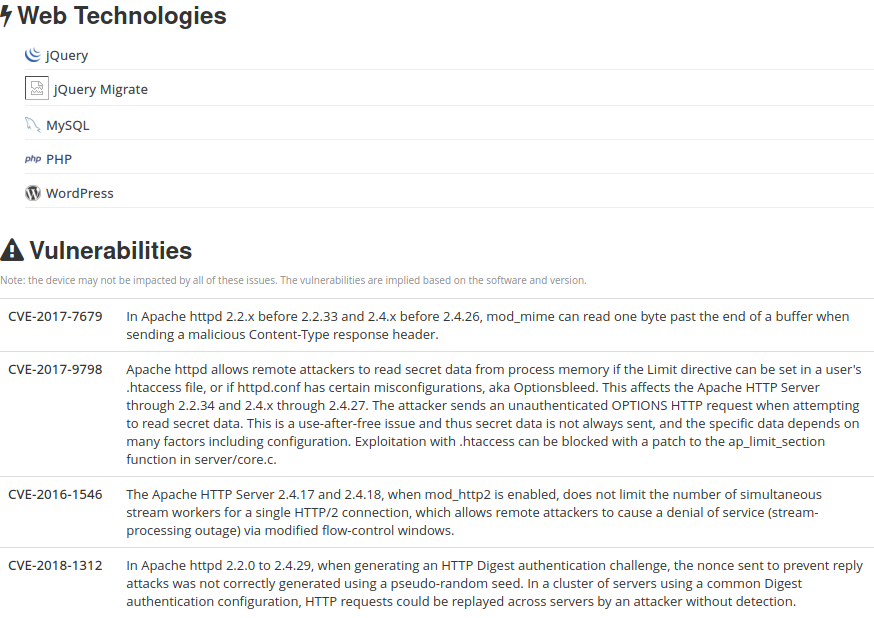
\includegraphics[scale=0.25]{shodan3.png}
  \caption{Detalle de resultados con Shodan sobre el host multimedia.uoc.edu (213.73.35.33)}
  \label{fig:otg-info-002-2}
\end{figure}

\pagebreak

\begin{figure}[h!]
  \centering
  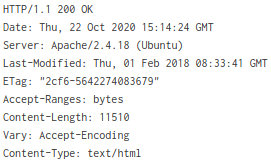
\includegraphics[scale=0.5]{headers.png}
  \caption{Resultados con Shodan sobre uoc.edu en el puerto 80}
  \label{fig:otg-info-002-2}
\end{figure}

\begin{figure}[h!]
  \centering
  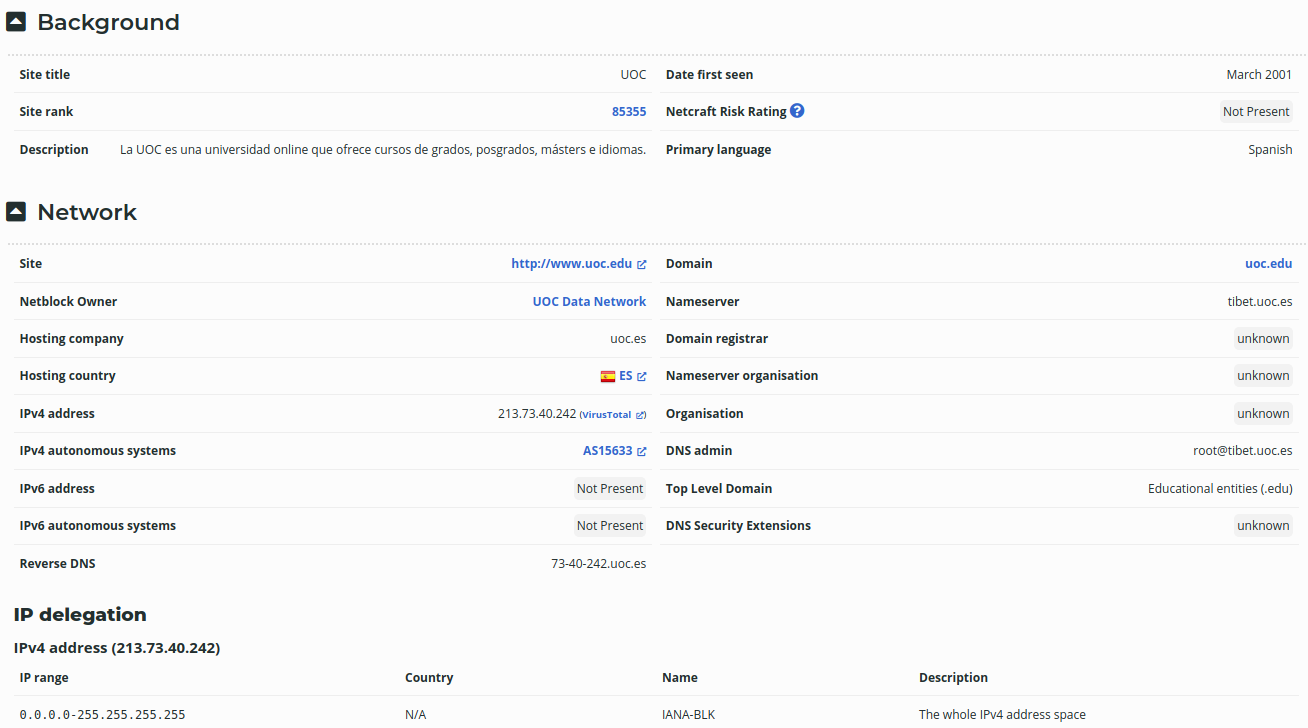
\includegraphics[scale=0.25]{netcraft.png}
  \caption{Resultados de la búsqueda de uoc.edu en Netcraft}
  \label{fig:otg-info-002-3}
\end{figure}

\pagebreak
\subsection{OTG-INFO-003}
\label{ann:otg-info-003}
\begin{figure}[h!]
  \centering
  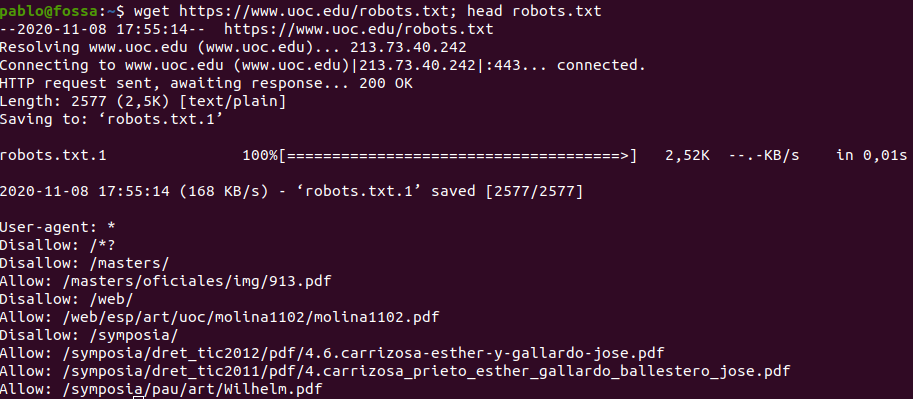
\includegraphics[scale=0.25]{robots.png}
  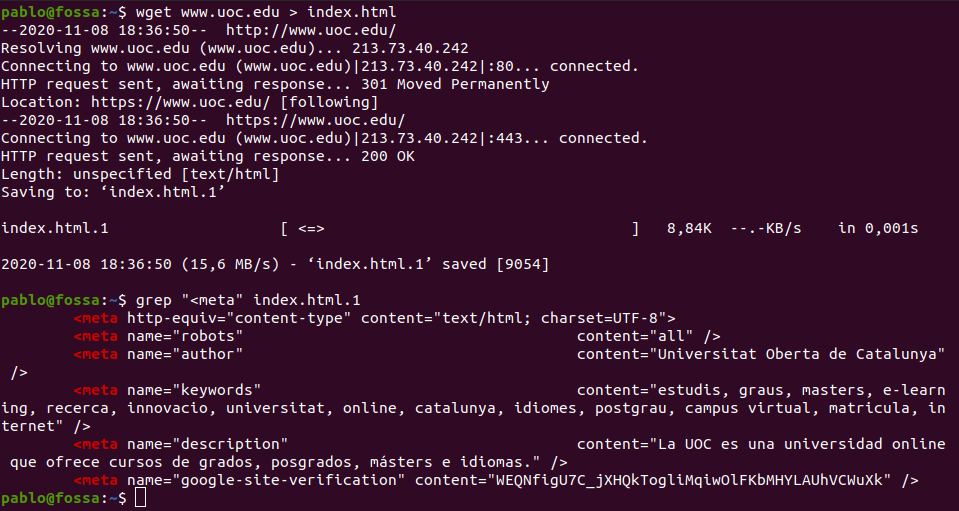
\includegraphics[scale=0.25]{meta.png}
  \caption{Listado de archivos de robots.txt y análisis de tags meta en el index.html}
  \label{fig:otg-info-003}
\end{figure}

\pagebreak

\subsection{OTG-INFO-004}
\label{ann:otg-info-004}
\begin{figure}[h!]
  \centering
  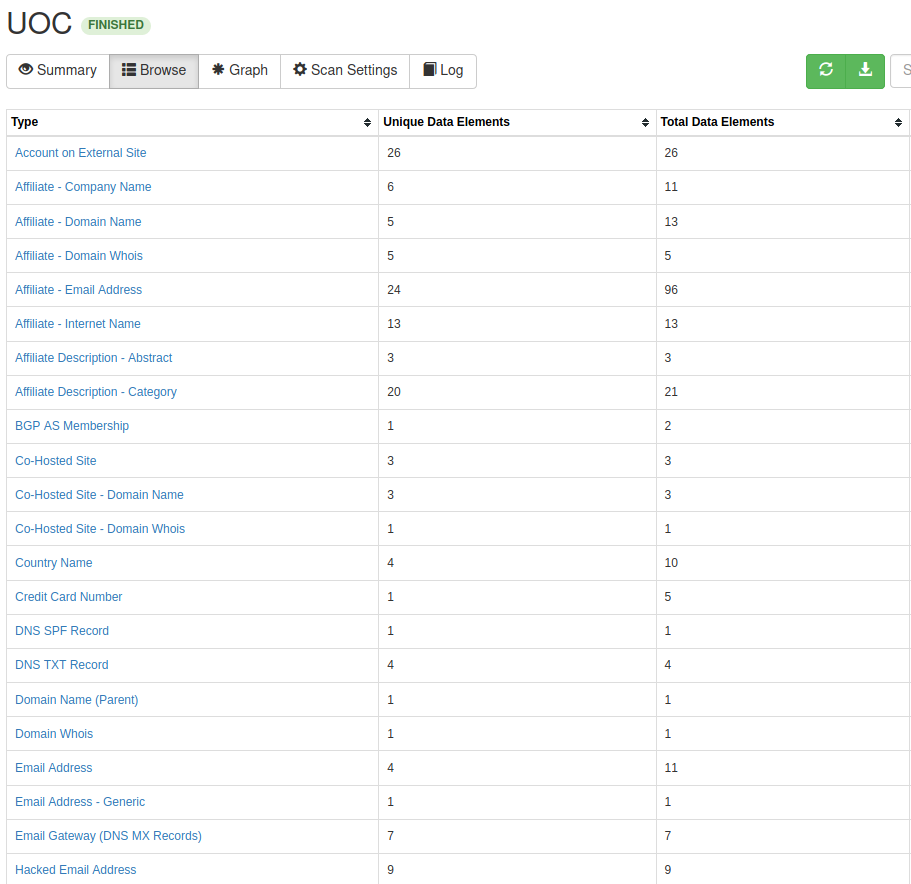
\includegraphics[scale=0.25]{spider2.png}
  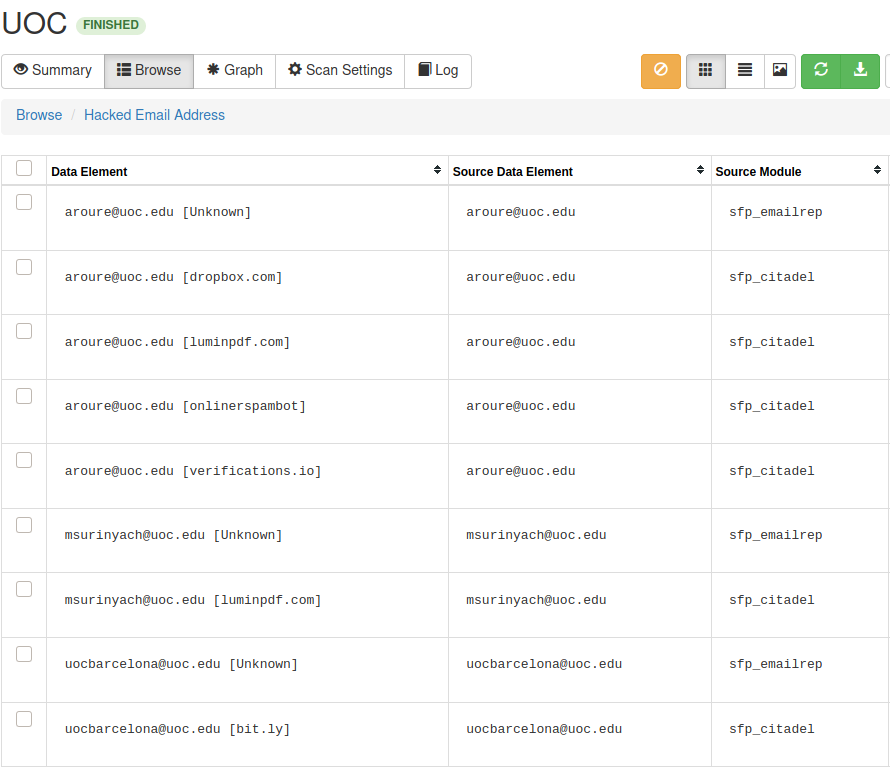
\includegraphics[scale=0.25]{hacked.png}
  \caption{SpiderFoot saca información relevante del dominio, incluído algunas cuentas de email que pertencen a fugas de datos.}
  \label{fig:otg-info-004-1}
\end{figure}

\begin{figure}[h!]
  \centering
  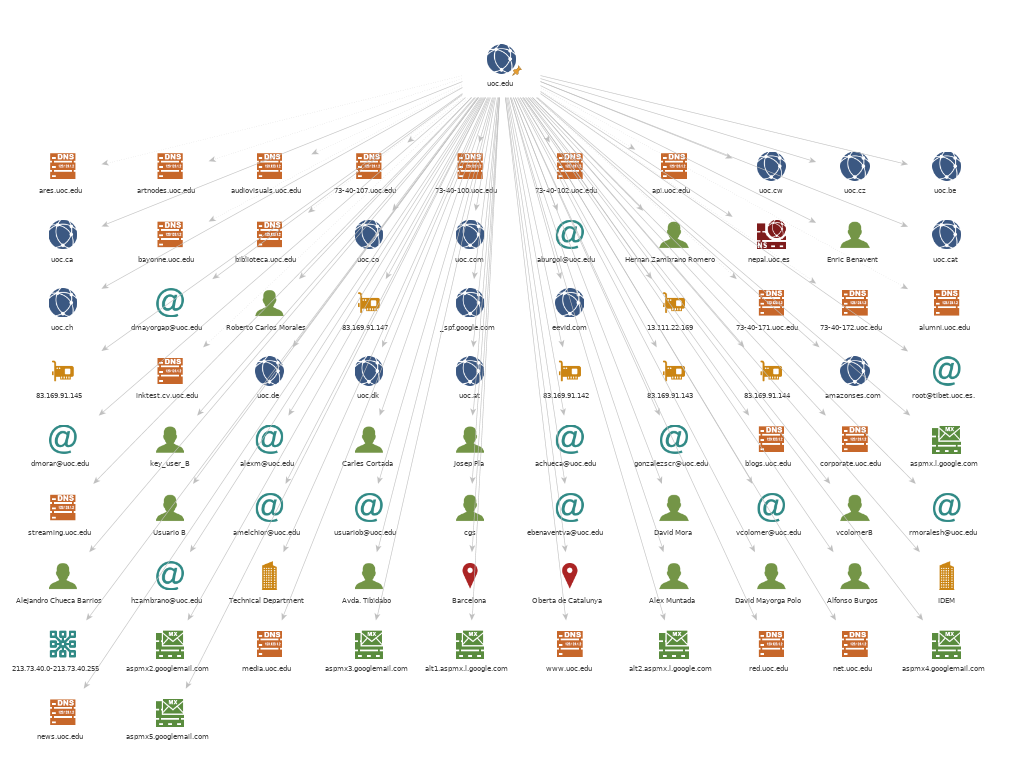
\includegraphics[scale=0.4]{maltego.png}
  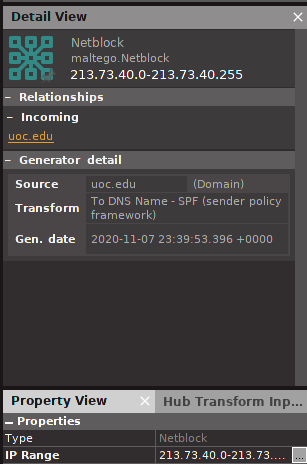
\includegraphics[scale=0.4]{maltego2.png}
  \caption{Grafo de Maltego sobre el dominio de uoc.edu y vista en detalle del bloque de red encontrado}
  \label{fig:otg-info-004-2}
\end{figure}

\begin{figure}[h!]
  \centering
  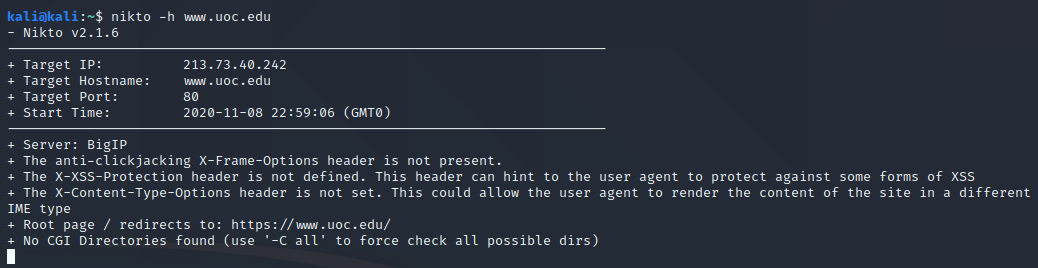
\includegraphics[scale=0.4]{nikto.png}
  \caption{Escaneo de la web por parte de Nikto}
  \label{fig:otg-info-004-3}
\end{figure}

\pagebreak
\subsubsection{nmap scan}
\label{ann:nmap}
\lstinputlisting[language=Python, firstline=10, lastline=34]{nmap_iprange.txt}
\vdots
\lstinputlisting[language=Python, firstline=252]{nmap_iprange.txt}

\pagebreak
\subsection{OTG-INFO-007}
\label{ann:otg-info-007}
\begin{figure}[h!]
  \centering
  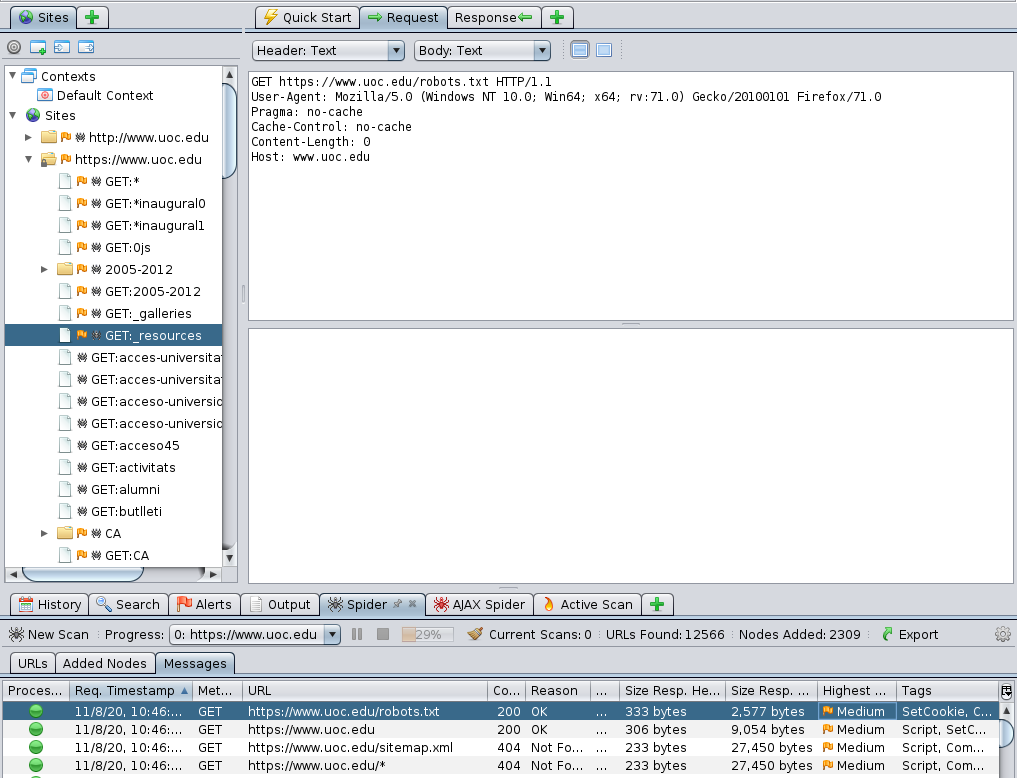
\includegraphics[scale=0.4]{zap1.png}
  \caption{Resultados de ZAP sobre el dominio www.uoc.edu. Muestra la request de tipo GET sobre el recurso robots.txt}
  \label{fig:otg-info-007-1}
\end{figure}

\begin{figure}[h!]
  \centering
  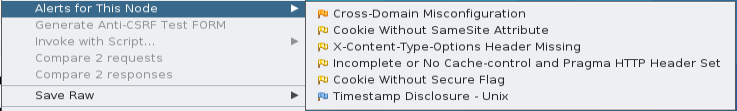
\includegraphics[scale=0.4]{zap2.png}
  \caption{Alertas detectadas para este nodo}
  \label{fig:otg-info-007-2}
\end{figure}

\subsection{OTG-INFO-008}
\label{ann:otg-info-008}

\begin{figure}[h!]
  \centering
  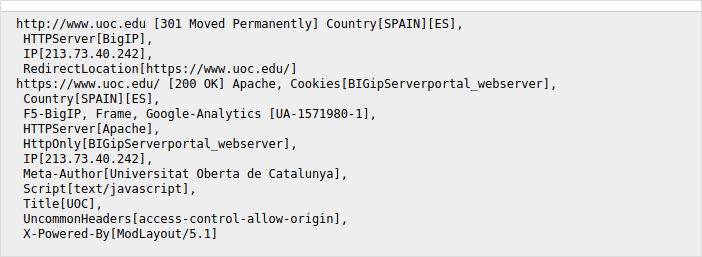
\includegraphics[scale=0.5]{whatweb.png}
  \caption{Análisis de fingerprinting del framework con whatweb}
  \label{fig:otg-info-008-1}
\end{figure}

\begin{figure}[h!]
  \centering
  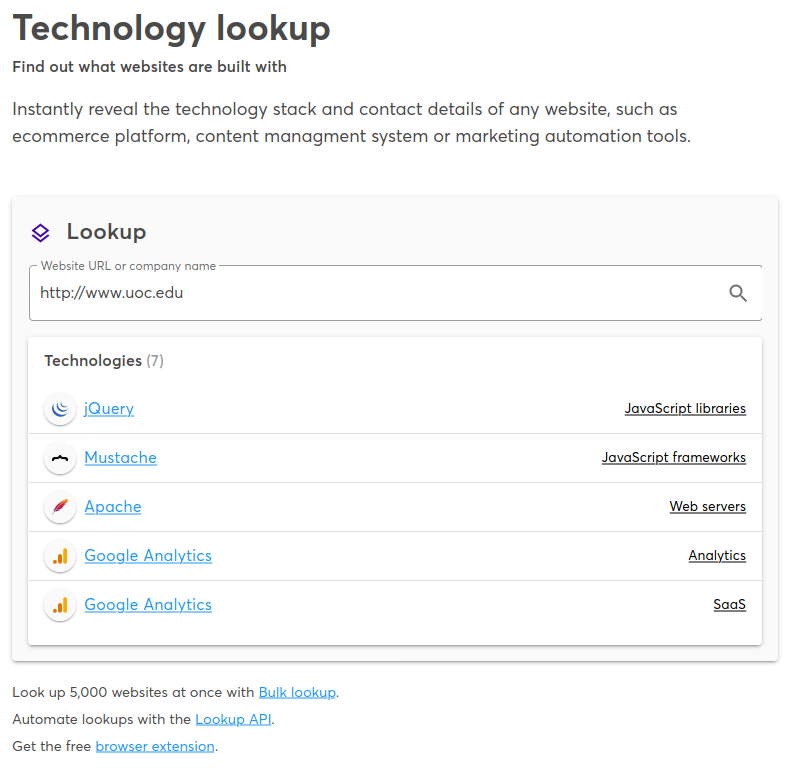
\includegraphics[scale=0.5]{wappalyzer.png}
  \caption{Análisis de fingerprinting del framework con wappalyzer}
  \label{fig:otg-info-008-2}
\end{figure}

\subsection{OTG-INFO-009}
\label{ann:otg-info-009}
\begin{figure}[h!]
  \centering
  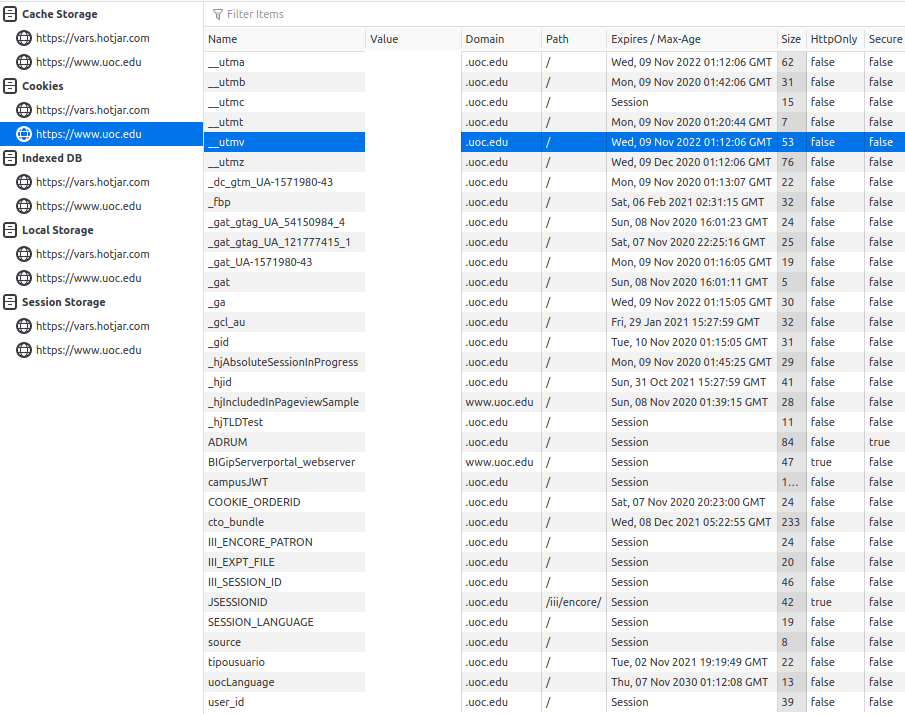
\includegraphics[scale=0.3]{cookies.png}
  \caption{Cookies de la página web}
  \label{fig:otg-info-009}
\end{figure}

\pagebreak

\begin{thebibliography}{9}

\bibitem{owasp}
	\textbf{Testing Information Gathering}\\
	\textit{OWASP}\\
	\url{https://wiki.owasp.org/index.php/Testing_Information_Gathering}

\bibitem{shodan}
	\textbf{What is Shodan?}\\
	\textit{Shodan - Help Center}\\
	\url{https://help.shodan.io/the-basics/what-is-shodan}

\bibitem{netcraft}
	\textbf{Search Web by Domain}\\
	\textit{Netcraft}\\
	\url{https://searchdns.netcraft.com/}
	
\bibitem{maltego}
	\textbf{Maltego is an open source intelligence (OSINT) and graphical link analysis tool for gathering and connecting information for investigative tasks.}\\
	\textit{Malego}\\
	\url{https://www.maltego.com/}
	
\bibitem{zap}
	\textbf{Introducing ZAP}\\
	\textit{OWASP ZAP}\\
	\url{https://www.zaproxy.org/getting-started/}

\bibitem{spiderfoot}
	\textbf{SpiderFoot HX: OSINT for Professionals}\\
	\url{https://www.spiderfoot.net/hx/}
	
\bibitem{hackedemail}
	\textbf{SpiderFoot 2.12 includes many new modules, including SecurityTrails, ARIN and FullContact.com among a number of improvements and bug fixes.}\\
	\textit{SpiderFoot}\\
	\url{https://www.spiderfoot.net/spiderfoot-2-12-includes-many-new-modules/}

\bibitem{nmap}
	\textbf{Network exploration tool and security / port scanner}\\
	\textit{nmap}\\
	\url{https://nmap.org/}

\bibitem{nikto}
	\textbf{Nikto is an Open Source (GPL) web server scanner which performs comprehensive tests against web servers for multiple items}\\
	\textit{Nikto}\\
	\url{https://cirt.net/Nikto2}

\bibitem{whatweb}
	\textbf{Identify the technology stack that powers a website and explore the Web of Things}\\
	\textit{Whatweb}\\
	\url{http://www.morningstarsecurity.com/research/whatweb}

\bibitem{x-pow}
	\textbf{What does “x-powered by” mean?}\\
	\textit{Stack Overflow}\\
	\url{https://stackoverflow.com/questions/33580671/what-does-x-powered-by-mean}

\bibitem{wappalyzer}
	\textbf{Identify technologies on websites}\\
	\textit{Wappalyzer}\\
	\url{https://www.wappalyzer.com/}

\bibitem{gaq}
	\textbf{What is var \_gaq = \_gaq $\vert \vert$ [ ]; for?}\\
	\textit{Stack Overflow}\\
	\url{https://stackoverflow.com/questions/2538252/what-is-var-gaq-gaq-for}

\end{thebibliography}

\end{document}